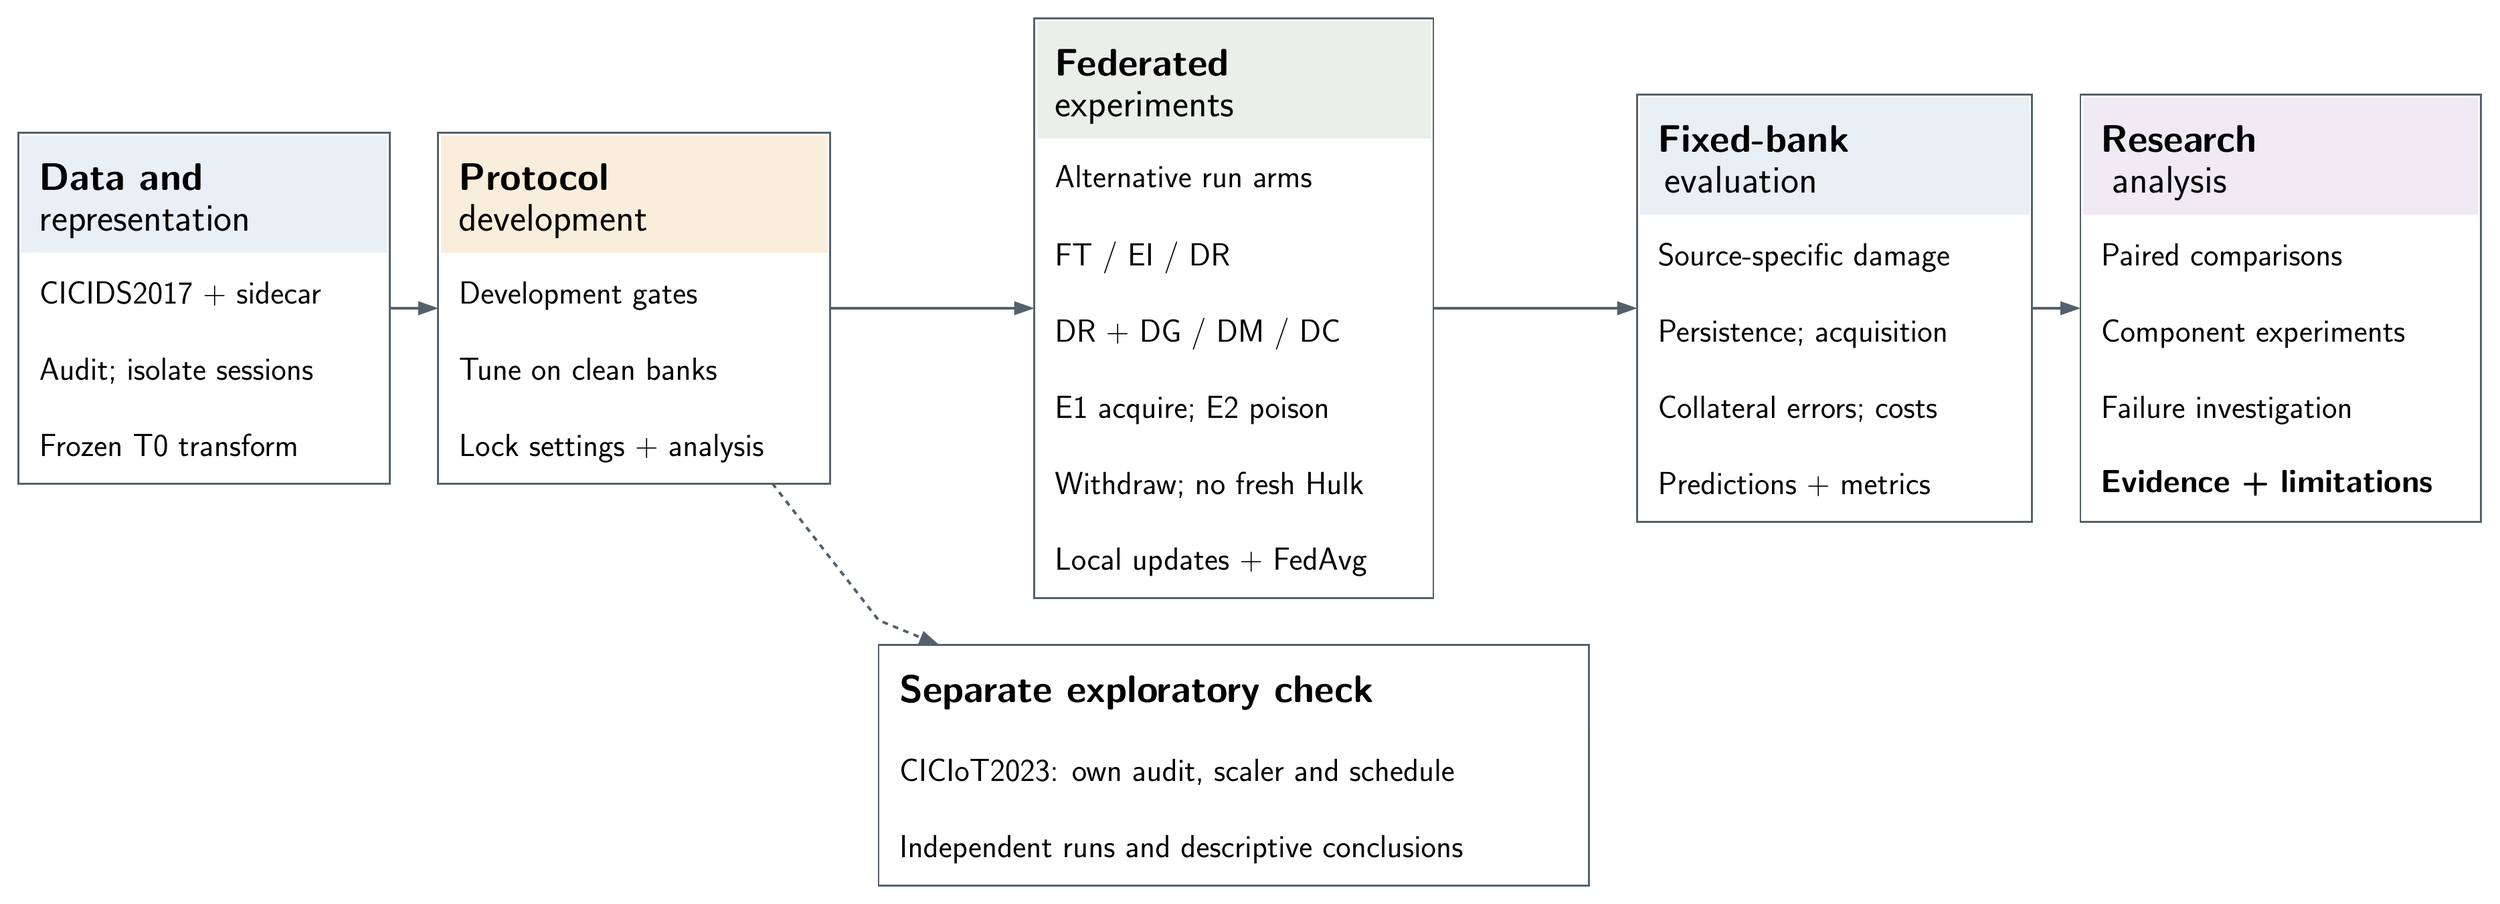
\begin{tikzpicture}[x=1bp,y=1bp]
\path[use as bounding box] (0,0) rectangle (1324.800,466.750);
\path[draw={rgb,255:red,84;green,97;blue,109},line width=1.4bp] (199.480,310.750) .. controls (204.950,310.750) and (210.460,310.750) .. (215.970,310.750);
\path[draw={rgb,255:red,84;green,97;blue,109},line width=1.4bp,fill={rgb,255:red,84;green,97;blue,109}] (215.760,313.550) -- (223.760,310.750) -- (215.760,307.950) -- cycle;
\path[draw={rgb,255:red,84;green,97;blue,109},line width=1.4bp] (436.310,310.750) .. controls (468.280,310.750) and (503.660,310.750) .. (536.400,310.750);
\path[draw={rgb,255:red,84;green,97;blue,109},line width=1.4bp,fill={rgb,255:red,84;green,97;blue,109}] (536.350,313.550) -- (544.350,310.750) -- (536.350,307.950) -- cycle;
\path[draw={rgb,255:red,84;green,97;blue,109},line width=1.4bp] (760.830,310.750) .. controls (792.880,310.750) and (828.210,310.750) .. (860.830,310.750);
\path[draw={rgb,255:red,84;green,97;blue,109},line width=1.4bp,fill={rgb,255:red,84;green,97;blue,109}] (860.730,313.550) -- (868.730,310.750) -- (860.730,307.950) -- cycle;
\path[draw={rgb,255:red,84;green,97;blue,109},line width=1.4bp] (1083.080,310.750) .. controls (1088.530,310.750) and (1094.020,310.750) .. (1099.500,310.750);
\path[draw={rgb,255:red,84;green,97;blue,109},line width=1.4bp,fill={rgb,255:red,84;green,97;blue,109}] (1099.230,313.550) -- (1107.230,310.750) -- (1099.230,307.950) -- cycle;
\path[draw={rgb,255:red,84;green,97;blue,109},line width=1.4bp,dashed] (405.510,216.440) .. controls (435.260,178.140) and (462.750,142.750) .. (462.750,142.750) .. controls (462.750,142.750) and (471.980,138.960) .. (486.370,133.050);
\path[draw={rgb,255:red,84;green,97;blue,109},line width=1.4bp,fill={rgb,255:red,84;green,97;blue,109}] (487.110,135.770) -- (493.450,130.150) -- (484.990,130.590) -- cycle;
\path[draw={rgb,255:red,255;green,255;blue,254},line width=1.0bp,fill={rgb,255:red,232;green,239;blue,245}] (1.000,340.250) -- (1.000,404.250) -- (198.750,404.250) -- (198.750,340.250) -- cycle;
\node[anchor=base west,inner sep=0,text={rgb,255:red,0;green,0;blue,0},font=\sffamily\bfseries\fontsize{22.0}{25.299999999999997}\selectfont] at (11.000,374.350) {Data and};
\node[anchor=base west,inner sep=0,text={rgb,255:red,0;green,0;blue,0},font=\sffamily\fontsize{22.0}{25.299999999999997}\selectfont] at (11.000,352.350) {representation};
\node[anchor=base west,inner sep=0,text={rgb,255:red,0;green,0;blue,0},font=\sffamily\fontsize{18.0}{20.7}\selectfont] at (11.000,313.150) {CICIDS2017 + sidecar};
\node[anchor=base west,inner sep=0,text={rgb,255:red,0;green,0;blue,0},font=\sffamily\fontsize{18.0}{20.7}\selectfont] at (11.000,272.150) {Audit; isolate sessions};
\node[anchor=base west,inner sep=0,text={rgb,255:red,0;green,0;blue,0},font=\sffamily\fontsize{18.0}{20.7}\selectfont] at (11.000,231.150) {Frozen T0 transform};
\path[draw={rgb,255:red,84;green,97;blue,109},line width=1.0bp] (0.000,216.250) -- (0.000,405.250) -- (199.750,405.250) -- (199.750,216.250) -- cycle;
\path[draw={rgb,255:red,255;green,255;blue,254},line width=1.0bp,fill={rgb,255:red,248;green,238;blue,219}] (226.750,340.250) -- (226.750,404.250) -- (435.750,404.250) -- (435.750,340.250) -- cycle;
\node[anchor=base west,inner sep=0,text={rgb,255:red,0;green,0;blue,0},font=\sffamily\bfseries\fontsize{22.0}{25.299999999999997}\selectfont] at (236.750,374.350) {Protocol};
\node[anchor=base west,inner sep=0,text={rgb,255:red,0;green,0;blue,0},font=\sffamily\fontsize{22.0}{25.299999999999997}\selectfont] at (236.750,352.350) {development};
\node[anchor=base west,inner sep=0,text={rgb,255:red,0;green,0;blue,0},font=\sffamily\fontsize{18.0}{20.7}\selectfont] at (236.750,313.150) {Development gates};
\node[anchor=base west,inner sep=0,text={rgb,255:red,0;green,0;blue,0},font=\sffamily\fontsize{18.0}{20.7}\selectfont] at (236.750,272.150) {Tune on clean banks};
\node[anchor=base west,inner sep=0,text={rgb,255:red,0;green,0;blue,0},font=\sffamily\fontsize{18.0}{20.7}\selectfont] at (236.750,231.150) {Lock settings + analysis};
\path[draw={rgb,255:red,84;green,97;blue,109},line width=1.0bp] (225.750,216.250) -- (225.750,405.250) -- (436.750,405.250) -- (436.750,216.250) -- cycle;
\path[draw={rgb,255:red,255;green,255;blue,254},line width=1.0bp,fill={rgb,255:red,233;green,239;blue,233}] (547.380,401.750) -- (547.380,465.750) -- (760.120,465.750) -- (760.120,401.750) -- cycle;
\node[anchor=base west,inner sep=0,text={rgb,255:red,0;green,0;blue,0},font=\sffamily\bfseries\fontsize{22.0}{25.299999999999997}\selectfont] at (557.380,435.850) {Federated};
\node[anchor=base west,inner sep=0,text={rgb,255:red,0;green,0;blue,0},font=\sffamily\fontsize{22.0}{25.299999999999997}\selectfont] at (557.380,413.850) {experiments};
\node[anchor=base west,inner sep=0,text={rgb,255:red,0;green,0;blue,0},font=\sffamily\fontsize{18.0}{20.7}\selectfont] at (557.380,375.650) {Alternative run arms};
\node[anchor=base west,inner sep=0,text={rgb,255:red,0;green,0;blue,0},font=\sffamily\fontsize{18.0}{20.7}\selectfont] at (557.380,333.650) {FT / EI / DR};
\node[anchor=base west,inner sep=0,text={rgb,255:red,0;green,0;blue,0},font=\sffamily\fontsize{18.0}{20.7}\selectfont] at (557.380,292.650) {DR + DG / DM / DC};
\node[anchor=base west,inner sep=0,text={rgb,255:red,0;green,0;blue,0},font=\sffamily\fontsize{18.0}{20.7}\selectfont] at (557.380,251.650) {E1 acquire; E2 poison};
\node[anchor=base west,inner sep=0,text={rgb,255:red,0;green,0;blue,0},font=\sffamily\fontsize{18.0}{20.7}\selectfont] at (557.380,210.650) {Withdraw; no fresh Hulk};
\node[anchor=base west,inner sep=0,text={rgb,255:red,0;green,0;blue,0},font=\sffamily\fontsize{18.0}{20.7}\selectfont] at (557.380,169.650) {Local updates + FedAvg};
\path[draw={rgb,255:red,84;green,97;blue,109},line width=1.0bp] (546.380,154.750) -- (546.380,466.750) -- (761.120,466.750) -- (761.120,154.750) -- cycle;
\path[draw={rgb,255:red,255;green,255;blue,254},line width=1.0bp,fill={rgb,255:red,232;green,239;blue,245}] (871.750,360.750) -- (871.750,424.750) -- (1082.250,424.750) -- (1082.250,360.750) -- cycle;
\node[anchor=base west,inner sep=0,text={rgb,255:red,0;green,0;blue,0},font=\sffamily\bfseries\fontsize{22.0}{25.299999999999997}\selectfont] at (881.750,394.850) {Fixed-bank};
\node[anchor=base west,inner sep=0,text={rgb,255:red,0;green,0;blue,0},font=\sffamily\fontsize{22.0}{25.299999999999997}\selectfont] at (885.500,372.850) {evaluation};
\node[anchor=base west,inner sep=0,text={rgb,255:red,0;green,0;blue,0},font=\sffamily\fontsize{18.0}{20.7}\selectfont] at (881.750,333.650) {Source-specific damage};
\node[anchor=base west,inner sep=0,text={rgb,255:red,0;green,0;blue,0},font=\sffamily\fontsize{18.0}{20.7}\selectfont] at (881.750,292.650) {Persistence; acquisition};
\node[anchor=base west,inner sep=0,text={rgb,255:red,0;green,0;blue,0},font=\sffamily\fontsize{18.0}{20.7}\selectfont] at (881.750,251.650) {Collateral errors; costs};
\node[anchor=base west,inner sep=0,text={rgb,255:red,0;green,0;blue,0},font=\sffamily\fontsize{18.0}{20.7}\selectfont] at (881.750,210.650) {Predictions + metrics};
\path[draw={rgb,255:red,84;green,97;blue,109},line width=1.0bp] (870.750,195.750) -- (870.750,425.750) -- (1083.250,425.750) -- (1083.250,195.750) -- cycle;
\path[draw={rgb,255:red,255;green,255;blue,254},line width=1.0bp,fill={rgb,255:red,239;green,234;blue,243}] (1110.250,360.750) -- (1110.250,424.750) -- (1323.750,424.750) -- (1323.750,360.750) -- cycle;
\node[anchor=base west,inner sep=0,text={rgb,255:red,0;green,0;blue,0},font=\sffamily\bfseries\fontsize{22.0}{25.299999999999997}\selectfont] at (1120.250,394.850) {Research};
\node[anchor=base west,inner sep=0,text={rgb,255:red,0;green,0;blue,0},font=\sffamily\fontsize{22.0}{25.299999999999997}\selectfont] at (1126.250,372.850) {analysis};
\node[anchor=base west,inner sep=0,text={rgb,255:red,0;green,0;blue,0},font=\sffamily\fontsize{18.0}{20.7}\selectfont] at (1120.250,333.650) {Paired comparisons};
\node[anchor=base west,inner sep=0,text={rgb,255:red,0;green,0;blue,0},font=\sffamily\fontsize{18.0}{20.7}\selectfont] at (1120.250,292.650) {Component experiments};
\node[anchor=base west,inner sep=0,text={rgb,255:red,0;green,0;blue,0},font=\sffamily\fontsize{18.0}{20.7}\selectfont] at (1120.250,251.650) {Failure investigation};
\node[anchor=base west,inner sep=0,text={rgb,255:red,0;green,0;blue,0},font=\sffamily\bfseries\fontsize{18.0}{20.7}\selectfont] at (1120.250,211.650) {Evidence + limitations};
\path[draw={rgb,255:red,84;green,97;blue,109},line width=1.0bp] (1109.250,195.750) -- (1109.250,425.750) -- (1324.750,425.750) -- (1324.750,195.750) -- cycle;
\path[draw={rgb,255:red,255;green,255;blue,254},line width=1.0bp,fill={rgb,255:red,255;green,255;blue,255}] (463.750,83.000) -- (463.750,128.500) -- (843.750,128.500) -- (843.750,83.000) -- cycle;
\node[anchor=base west,inner sep=0,text={rgb,255:red,0;green,0;blue,0},font=\sffamily\bfseries\fontsize{22.0}{25.299999999999997}\selectfont] at (473.750,98.600) {Separate exploratory check};
\node[anchor=base west,inner sep=0,text={rgb,255:red,0;green,0;blue,0},font=\sffamily\fontsize{18.0}{20.7}\selectfont] at (473.750,55.900) {CICIoT2023: own audit, scaler and schedule};
\node[anchor=base west,inner sep=0,text={rgb,255:red,0;green,0;blue,0},font=\sffamily\fontsize{18.0}{20.7}\selectfont] at (473.750,14.900) {Independent runs and descriptive conclusions};
\path[draw={rgb,255:red,84;green,97;blue,109},line width=1.0bp] (462.750,0.000) -- (462.750,129.500) -- (844.750,129.500) -- (844.750,0.000) -- cycle;
\end{tikzpicture}